\section{Physics Options}
\label{sec:physics_options}
The Physics Options tab contains settings which control gravitational and \ac{SRP} effects on the spacecraft including how \ac{EMTG} computes the ephemerides for bodies in the mission Universe. Settings for the \ac{EMTG} integrator (if used) are also available on this tab. These options effect \ac{EMTG}'s accuracy, run time, and memory requirements. Additional settings for how \ac{EMTG} represents states for periapse boundaries and parallel shooting constraints and decision variables are also controlled from this tab. 

\noindent When changing settings on this tab, keep in mind that certain options only take effect when the appropriate mission type is selected for each Journey. This section and Chapters \ref{chap:force_model_prop} and \ref{chap:mission_types} should be referenced together when selecting appropriate settings for the mission design.

    \begin{figure}[H]
        \centering
        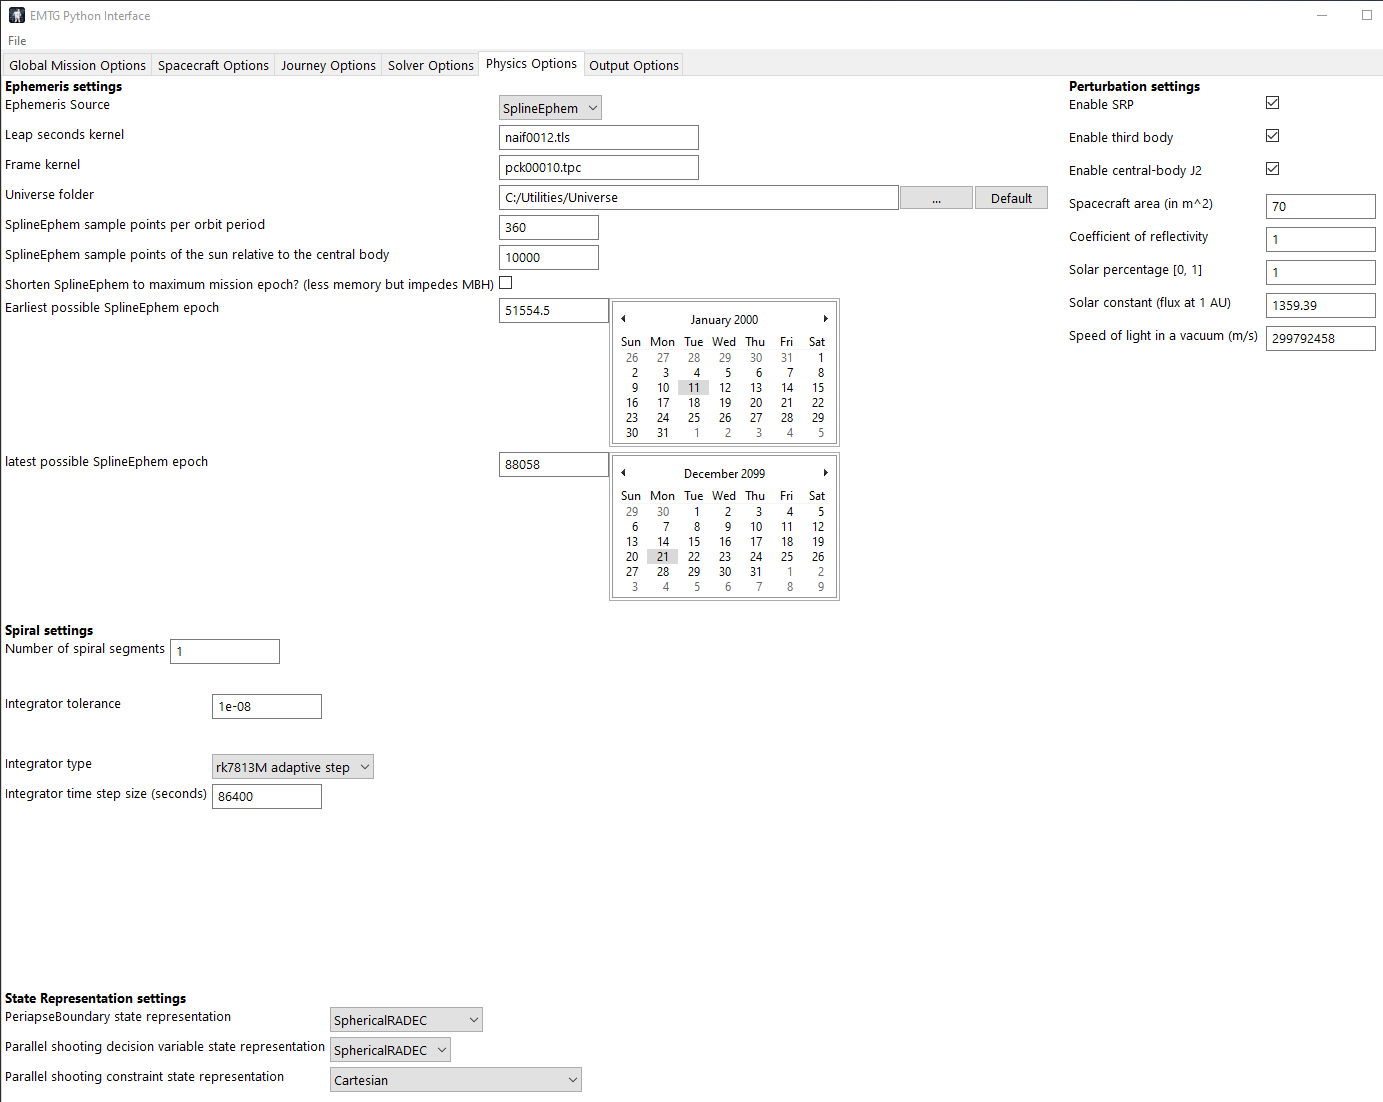
\includegraphics[width=1.0\textwidth]{../../shared_latex_inputs/images/pyemtg_physics_options_tab.png}
        \caption{EMTG Physics Options tab}
    \end{figure}

\subsection{Ephemeris Settings}
The Ephemeris settings control how \ac{EMTG} uses \ac{SPICE} to generate ephemeris states for Universe file bodies. For speed reasons \ac{EMTG} by default does not call the \ac{SPICE} library directly each time it needs a body state, but instead builds a set of ephemeris interpolations using cubic spline functions.

    \begin{figure}[H]
        \centering
        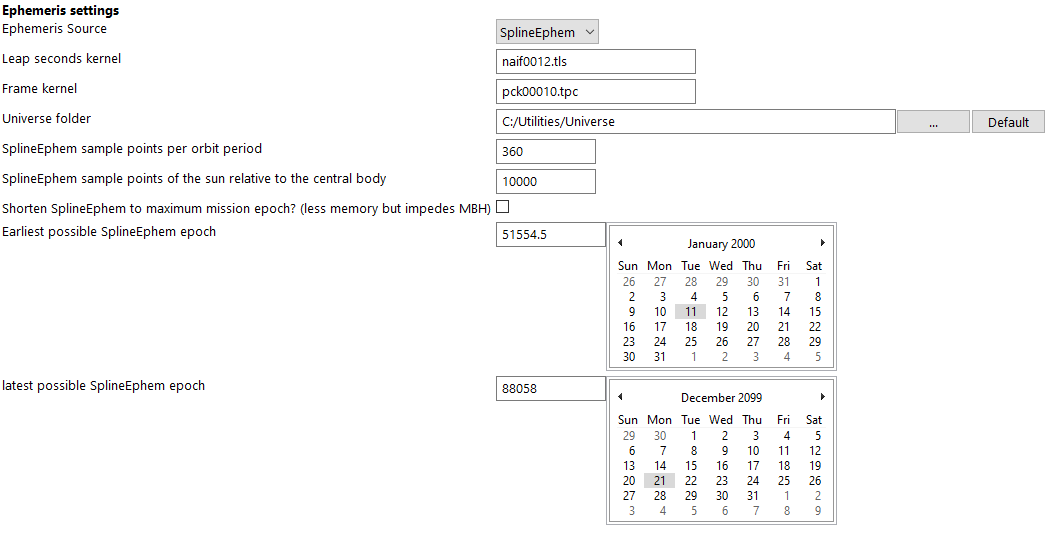
\includegraphics[width=0.9\textwidth]{../../shared_latex_inputs/images/pyemtg_physics-ephem_options.png}
        \caption{EMTG Physics Options - Ephemeris Settings}
    \end{figure}

    \begin{enumerate}

        \item \textbf{Ephemeris Source:} Select the method \ac{EMTG} uses to get body ephemeris. \verb|SplineEphem| is the fastest method relying on cubic spline functions. It requires additional memory than other methods but also provides analytical partial derivatives. \verb|\ac{SPICE}| calls the CSPICE library each time ephemeris information is required. This method is slower and relies on finite differencing for derivatives but uses less memory. It is also slightly more accurate.
        % #TODO what does static do?

            \begin{table}[H]
                \hspace{2cm}
                \begin{tabular}{ll}
                Data Type & \verb|int| \\
                Allowed Values & 0: \verb|Static|, 1: \verb|\ac{SPICE}|, 2: \verb|SplineEphem| \\
                Default Value & 2: \verb|SplineEphem| \\
                \end{tabular}
            \end{table}

        \item \textbf{Leap seconds kernel:} Leap seconds kernel file to use. The file should be located in the Universe folder specified using the setting below. Leap second kernels can be found on the \href{https://naif.jpl.nasa.gov/naif/data_generic.html}{JPL NAIF website.}

            \begin{table}[H]
                \hspace{2cm}
                \begin{tabular}{ll}
                Data Type & \verb|string| \\
                Default Value & ``naif0012.tls'' \\
                \end{tabular}
            \end{table}

        \item \textbf{Frame kernel:} Frame kernel file to use. The file should be located in the Universe folder specified using the setting below. Frame kernels can be found on the \href{https://naif.jpl.nasa.gov/naif/data_generic.html}{JPL NAIF website.}

            \begin{table}[H]
                \hspace{2cm}
                \begin{tabular}{ll}
                Data Type & \verb|string| \\
                Default Value & ``pck00010.tpc'' \\
                \end{tabular}
            \end{table}
    
        \item \textbf{SplineEphem sample points per orbit period:} This setting controls the number of points drawn from \ac{SPICE} per period of the central body which allows the user control the accuracy and memory footprint of the spline.
        
            \begin{table}[H]
                \hspace{2cm}
                \begin{tabular}{ll}
                Data Type & \verb|int| \\
                Allowed Values & 1 $<$ Integer $<$ $\infty$ \\
                Default Value & 360 \\
                Units & NA
                \end{tabular}
            \end{table}

        \item \textbf{SplineEphem sample points of the sun relative to the central body:}This setting controls the number of points drawn from \ac{SPICE} for the sun relative to the central body.
        
            \begin{table}[H]
                \hspace{2cm}
                \begin{tabular}{ll}
                Data Type & \verb|int| \\
                Allowed Values & 1 $<$ Integer $<$ $\infty$ \\
                Default Value & 360 \\
                Units & NA
                \end{tabular}
            \end{table}

        \item \textbf{Shorten SplineEphem to maximum mission epoch?:} Sets the upper bound on the \ac{SPICE} ephemeris splines to the global flight time bounds set in the Global Mission Options tab see Section \ref{sec:global_options}. Reduces \ac{EMTG}'s memory requirements. The lower bound is decreased by ten days and the upper bound is increased by ten days to ensure the splines are well-defined at the global flight time bounds.

            \begin{table}[H]
                \hspace{2cm}
                \begin{tabular}{ll}
                Data Type & \verb|bool| \\
                Allowed Values & true, false \\
                Default Value & false \\
                Units & NA
                \end{tabular}
            \end{table}

        \item \textbf{Earliest/Latest possible SplineEphem epoch:} Sets epoch bounds on the \ac{SPICE} ephemeris splines when \verb|SplineEphem| is used as the ephemeris source. Reduces \ac{EMTG}'s memory requirements. The lower bound is decreased by ten days and the upper bound is increased by ten days to ensure the splines are well-defined at the epoch bounds.
                
            \begin{table}[H]
                \hspace{2cm}
                \begin{tabular}{ll}
                Data Type & \verb|double| \\
                Allowed Values & 33251 (1 DEC 1949) $<$ Real $<$ 100000 (31 AUG 2132)\\
                Default Value & 51554.5 (11 JAN 2000) (Earliest) and 88058 (21 DEC 2099) (Latest)\\
                Units & days
                \end{tabular}
            \end{table}
    
    \end{enumerate}

\subsection{Spiral Settings}

    \begin{enumerate}

        \item \textbf{Number of spiral segments:} Sets the number of spiral segments when using Journey departure type, ``5: Spiral-out from circular orbit'' or Journey arrival type ``6: capture spiral.'' \ac{EMTG} uses Edelbaum's spiral approximation to approximate a many-revolution low-thrust spiral about a body. See sections \ref{sec:capture_spiral} and \ref{sec:spiral_out} for more information about Journey spiral arrival and departure.
        
            \begin{table}[H]
                \hspace{2cm}
                \begin{tabular}{ll}
                Data Type & \verb|int| \\
                Allowed Values & 1 $<$ Integer $<$ $\infty$ \\
                Default Value & 1 \\
                Units & NA
                \end{tabular}
            \end{table}
    
    \end{enumerate}

\subsection{Integrator Settings}

    This section contains the settings for \ac{EMTG}'s numerical integrators. Note that not all mission types use numerical integration for propagation of the spacecraft. If using Keplerian propagation, the integration options set here will have no effect. Refer to chapter \ref{chap:mission_types} for a discussion of the different Mission Types and propagation methods they use.

    \begin{enumerate}

        \item \textbf{Integrator tolerance:} Sets the maximum allowable error in the numerical solution of the ordinary differential equation (ODE)
        
            \begin{table}[H]
                \hspace{2cm}
                \begin{tabular}{ll}
                Data Type & \verb|double| \\
                Allowed Values & 1.0E-12 $<$ Real $<$ 1 \\
                Default Value & 1.0E-8 \\
                Units & NA
                \end{tabular}
            \end{table}

        \item \textbf{Integrator type:} Select the integrator type. Currently limited to a Runge-Kutta 8th order fixed step size method. Additional integrator methods may be implemented in the future and optionally selected here.
        % Choose from either a Runge-Kutta 8th order 8(7)13M adaptive step (note that the work by Prince and Dormand refer to this integration as 8(7)13M while PyEMTG refers to it as rk7813M) or a Runge-Kutta 8th order fixed step size. Currently only \verb|rk8 fixed step| works in \ac{EMTG}. Do not select \verb|rk7813M adaptive step| as it has not been fully implemented.
        
            \begin{table}[H]
                \hspace{2cm}
                \begin{tabular}{ll}
                Data Type & \verb|(IntegratorType) int| \\
                Allowed Values & \verb|0: rk7813M adaptive step, 1: rk8 fixed step|  \\
                Default Value & 1 \\
                \end{tabular}
            \end{table}

            % #TODO citation:
            % P.J. Prince, J.R. Dormand,
            % High order embedded Runge-Kutta formulae,
            % Journal of Computational and Applied Mathematics,
            % Volume 7, Issue 1,
            % 1981,
            % Pages 67-75,
            % ISSN 0377-0427,
            % https://doi.org/10.1016/0771-050X(81)90010-3.
            % (https://www.sciencedirect.com/science/article/pii/0771050X81900103)
        
        
        \item \textbf{Integrator time step size (seconds):}
            % #TODO what will EMTG do if it cannot maintain this step size?

            \begin{table}[H]
                \hspace{2cm}
                \begin{tabular}{ll}
                Data Type & \verb|double| \\
                Allowed Values & 1.0E-10 $<$ Real $<$ $\infty$ \\
                Default Value & 86400 \\
                Units & seconds
                \end{tabular}
            \end{table}

    \end{enumerate}

\subsection{State Representation Settings}

    This section allows the user additional control over \ac{EMTG}'s internal state representation. Typically \ac{EMTG}'s default state representation is cartesian. However for periapse boundary states and parallel shooting decision variables, the default state is spherical using right ascension and declination.

    \begin{figure}[H]
        \centering
        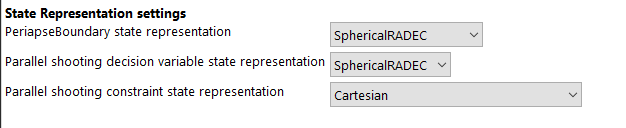
\includegraphics[width=0.9\textwidth]{../../shared_latex_inputs/images/pyemtg_physics-state_options.png}
        \caption{EMTG Physics Options - State Representation Settings}
    \end{figure}

    \begin{enumerate}

        \item \textbf{PeriapseBoundary state representation:} Allows the user to change \ac{EMTG}'s internal state representation for the \verb|PeriapseBoundary| class. See Section \ref{sec:periapse_boundary}
        
            \begin{table}[H]
                \hspace{2cm}
                \begin{tabular}{lp{3cm}}
                Data Type & \verb|(StateRepresentation) int| \\
                Allowed Values & \verb|0: Cartesian, 1: SphericalRADEC, 2: SphericalAZFPA,| \newline
                    \verb|3: COE, 4: MEE, 5: IncomingBplane, 6: OutgoingBplane,|\newline 
                    \verb|7: IncomingBplaneRpTA, 8: OutgoingBplaneRpTA|  \\
                Default Value & 1 \\
                \end{tabular}
            \end{table}

        \item \textbf{Parallel shooting decision variable state representation:}  Allows the user to change \ac{EMTG}'s internal state representation for parallel shooting mission type decision variables. See Sections \ref{sec:parallel_shooting_bounded_impulse} and \ref{sec:parallel_shooting_finite_burn} for more information on parallel shooting.
        
            \begin{table}[H]
                \hspace{2cm}
                \begin{tabular}{lp{3cm}}
                Data Type & \verb|(StateRepresentation) int| \\
                Allowed Values & \verb|0: Cartesian, 1: SphericalRADEC, 2: SphericalAZFPA,| \newline
                    \verb|3: COE, 4: MEE| \\
                Default Value & 1 \\
                \end{tabular}
            \end{table}
        
        \item \textbf{Parallel shooting constraint representation:}  Allows the user to change \ac{EMTG}'s constraint representation for parallel shooting mission type. See Section \ref{sec:parallel_shooting_bounded_impulse} for more information on parallel shooting.

            \begin{table}[H]
                \hspace{2cm}
                \begin{tabular}{lp{3cm}}
                Data Type & \verb|(ConstraintStateRepresentation) int| \\
                Allowed Values & \verb|0: Cartesian, 1: Same as encoded state representation| \\
                Default Value & 0 \\
                \end{tabular}
            \end{table}

    \end{enumerate}

\subsection{Perturbation Settings}

    \begin{figure}[H]
        \centering
        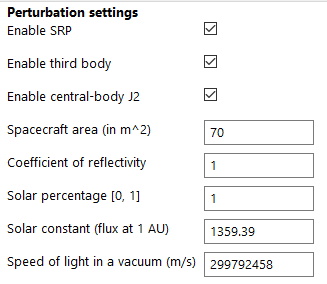
\includegraphics[width=0.5\textwidth]{../../shared_latex_inputs/images/pyemtg_physics-perturbation_options.png}
        \caption{EMTG Physics Options - Perturbation Settings}
    \end{figure}


    \begin{enumerate}

        \item \textbf{Enable \ac{SRP}:} Activate \ac{EMTG}'s spherical/cannonball solar radiation pressure (\ac{SRP}) model. Selecting this option will reveal additional configurable settings for \ac{EMTG}'s \ac{SRP} model: spacecraft area, coefficient of reflectivity, solar percentage, solar constant, and speed of light in a vacuum.
        
            \begin{table}[H]
                \hspace{2cm}
                \begin{tabular}{ll}
                Data Type & \verb|bool| \\
                Allowed Values & true, false \\
                Default Value & false \\
                Units & NA
                \end{tabular}
            \end{table}

        \item \textbf{Enable third body:} Activate third body gravitational perturbations. Selecting this option reveals a "Perturbation bodies" setting on the Journey Options tab allowing the user to select which bodies will contribute to third body accelerations on a per-Journey basis. Selecting this option turns on third body perturbations for all Journeys whose mission type and propagator supports perturbations, but only those bodies listed on the Journey page will contribute. See Chapter \ref{chap:mission_types} for more information.

            \begin{table}[H]
                \hspace{2cm}
                \begin{tabular}{ll}
                Data Type & \verb|bool| \\
                Allowed Values & true, false \\
                Default Value & false \\
                Units & NA
                \end{tabular}
            \end{table}

        \item \textbf{Enable central-body J2:} Activate J2 spherical harmonic gravitational forces for the central body of each Journey. For this force to be included, the Universe file for the central body must contain a value for J2 and a J2 reference radius (units of km) in the central body section of the Universe file. Like third body perturbations, central-body J2 activates J2 effects for all Journeys whose mission type and propagator supports perturbations. See Chapter \ref{chap:mission_types} for more information.

            \begin{table}[H]
                \hspace{2cm}
                \begin{tabular}{ll}
                Data Type & \verb|bool| \\
                Allowed Values & true, false \\
                Default Value & false \\
                Units & NA
                \end{tabular}
            \end{table}

        \item \textbf{Spacecraft area (in m\^{}2):} Set spacecraft cross-sectional area used to compute \ac{SRP} effects. Only active when ``enable \ac{SRP}'' is selected.

            \begin{table}[H]
                \hspace{2cm}
                \begin{tabular}{ll}
                Data Type & \verb|double| \\
                Allowed Values & 0 $<$ Real $<$ $\infty$ \\
                Default Value & 70 \\
                Units & $m^2$
                \end{tabular}
            \end{table}

        \item \textbf{Coefficient of reflectivity:} Set spacecraft coefficient of reflectivity used to compute \ac{SRP} effects. Only active when ``Enable \ac{SRP}'' is selected.

            \begin{table}[H]
                \hspace{2cm}
                \begin{tabular}{ll}
                Data Type & \verb|double| \\
                Allowed Values & 0 $<$ Real $<$ $\infty$ \\
                Default Value & 1 \\
                Units & NA
                \end{tabular}
            \end{table}

        \item \textbf{Solar percentage [0, 1]:} Set solar percentage used to compute \ac{SRP} effects. This setting combined with ``solar constant'' can be used to examine the effects of solar activity levels on the mission design. Only active when ``Enable \ac{SRP}'' is selected.
        
            \begin{table}[H]
                \hspace{2cm}
                \begin{tabular}{ll}
                Data Type & \verb|double| \\
                Allowed Values & 0 $<$ Real $<$ 1 \\
                Default Value & 1 \\
                Units & NA
                \end{tabular}
            \end{table}

        \item \textbf{Solar constant (flux at 1 AU):} Set solar flux at 1 AU used to compute \ac{SRP} effects. This setting combined with ``solar percentage'' can be used to examine the effects of solar activity levels on the mission design. Only active when ``Enable \ac{SRP}'' is selected.
        
            \begin{table}[H]
                \hspace{2cm}
                \begin{tabular}{ll}
                Data Type & \verb|double| \\
                Allowed Values & 0 $<$ Real $<$ $\infty$ \\
                Default Value & 1359.39 \\
                Units & $W/m^2$
                \end{tabular}
            \end{table}

        \item \textbf{Speed of light in a vacuum (m/s):} Set speed of light in a vacuum. This is normally left at it's default value.

        \begin{table}[H]
            \hspace{2cm}
            \begin{tabular}{ll}
            Data Type & \verb|double| \\
            Allowed Values & 0 $<$ Real $<$ $\infty$ \\
            Default Value & 299792458 \\
            Units & m/s
            \end{tabular}
        \end{table}

    \end{enumerate}